\documentclass{standalone}
\usepackage{tikz}
\usepackage{tikz-dimline}		% Dimension (measure) lines for TikZ
\usetikzlibrary{angles, calc, decorations.pathmorphing, quotes, spy}

\begin{document}
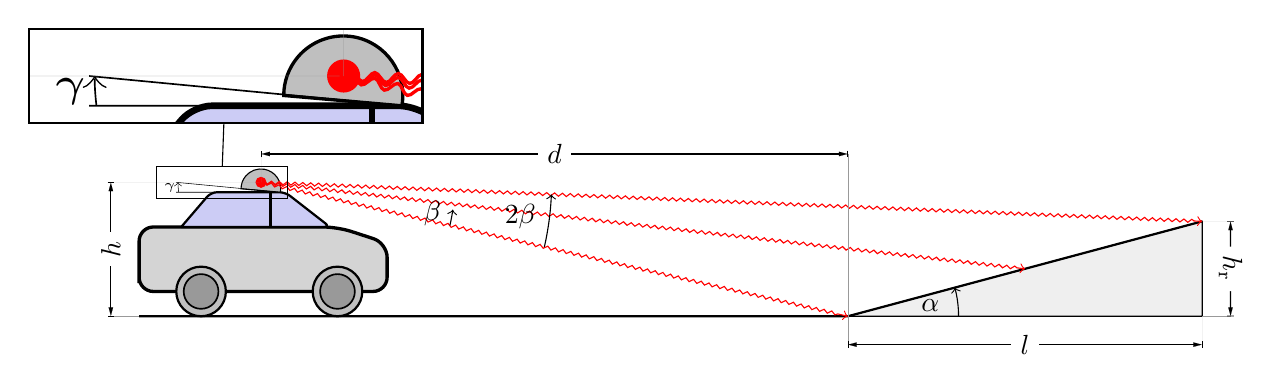
\begin{tikzpicture}[scale=0.9, spy using outlines={black, rectangle, magnification=3, width=5cm, height=1.2cm, connect spies}]
    % Define/Calc ramp parameters
    % Ramp length
    \def\rl{5};
    % Ramp angle [deg]
    \def\ra{15};
    % Ramp height
    \def\rh{{tan(\ra)*\rl}};
    % Distance of measurement line
    \def\dd{.4cm}

    % RAMP
    % Define the points
    \coordinate (A) at (0,0);
    \coordinate (B) at ($(A) + (\rl,0)$);
    \coordinate (C) at ($(B) + (0,\rh)$);
    % Draw and fill ramp
    \filldraw[draw=black, fill=lightgray!25] (A) -- (B) -- (C) -- cycle;
    % Draw angle
    \path (A) -- (B)
    pic[draw, ->, angle radius=40pt,
    angle eccentricity=0.75, "$\alpha$"]{angle=B--A--C};
    % Ground and helpers
    \coordinate (D) at ($(A) + (-10,0)$);
    \draw [thick] (D) -- (A) -- (C);

    % CAR
    \begin{scope}[scale=0.7]
        % Car height
        \def\ch{2}
        % Car length
        \def\cl{5}
        % Car body height
        \def\bh{\ch*0.65}
        % Roof length
        \def\rl{\cl*0.6}
        % Roof height
        \def\rh{\ch*0.35}
        % Car tilt angle
        \def\ct{6}
        % Anchor point is southwest
        \coordinate (b) at ($(D) + (0,0.5)$);
        % Offset to roof and wheels
        \coordinate (r) at ($(b) +(\cl*0.17,\ch*0.65)$);
        \coordinate (w) at ($(b) + (\cl*0.25,0)$);

        % Body
        \draw[black, fill=black!17, rounded corners=1.2ex, very thick]
        (b) -- ++(0,\bh) -- ++(\cl*1/5,0) --  ++(\cl*3/5,0) -- ++(\cl*1/5,-\bh*0.25)
        -- ++(0, -\bh*0.75) -- (b) -- cycle;
        % Roof
        \draw[very thick, rounded corners=0.5ex, fill=black!20!blue!20!white,thick]
        (r) -- ++(0.2*\rl,\rh) -- ++(0.5*\rl,0) -- ++(0.3*\rl,-\rh) -- (r);
        % \draw[thick] ($(r) + (\cl*0.5,\bh)$) -- ++(0,\rh);
        \draw[thick] (r)++(\rl*0.6,0) -- ++(0,\rh);

        % Wheels
        \draw[draw=black,fill=gray!50,thick] (w) circle (.5);
        \draw[draw=black,fill=gray!50,thick] (w) ++(\cl*0.55,0) circle (.5);
        % Inner wheels
        \draw[draw=black,fill=gray!80,semithick] (w) circle (.35);
        \draw[draw=black,fill=gray!80,semithick] (w) ++(\cl*0.55,0) circle (.35);

        % Lidar
        \draw[black, fill=gray!50] ($(r) + (\cl*0.40,\rh)$) coordinate (le) arc(-10:180:0.4) --cycle;

        % Car middle point
        \coordinate (m) at (\cl*0.5, \bh*0.5);
        % Lidar middle point
        \coordinate (lm) at ($(le) + (-0.39,0.2)$);
        \filldraw[red] (lm) circle(.1);
        % lidar mount angle
        % \draw (lm) -- ($(lm) + (-3, 0)$);
        % \path (A) -- (B)
        \coordinate (blob) at ($(le) + (-2.1, 0)$);
        \coordinate (blub) at ($(le) + (-2.1, 0.2)$);
        % \draw (blob) circle (.1);
        % \draw (blub) circle (.1);
        \draw[draw=black, very thin] (blob) -- (le) -- (blub)
        pic[draw, <-, angle radius=30pt,
        angle eccentricity=1.1, "\tiny $\gamma$"]{angle=blub--lm--blob};

        % Laser lines
        \draw[->,color=red,decorate,decoration={snake,amplitude=.2mm,segment length=1mm,post length=1mm}] (lm) -- (A);
        \draw[->,color=red,decorate,decoration={snake,amplitude=.2mm,segment length=1mm,post length=1mm}] (lm) -- ($(A)!0.5!(C)$);
        \draw[->,color=red,decorate,decoration={snake,amplitude=.2mm,segment length=1mm,post length=1mm}] (lm) -- ($(A)!1!(C)$);
        \path (lm) -- (A)
        pic[draw, ->, angle radius=70pt, angle eccentricity=0.9,
        "$\beta$"]{angle=A--lm--B};
        \path (lm) -- (C)
        pic[draw, ->, angle radius=105pt, angle eccentricity=0.9,
        "$2\beta$"]{angle=A--lm--C};
    \end{scope}

    % \dimline[extension start length=-\dd, extension end length=-\dd] {($(D)+(0,-\dd)$)}{($(A)+(0,-\dd)$)}{$d$};
    % \dimline[extension start length=\dd, extension end length=\dd] {($(A)+(0,-\dd)$)}{($(A)!0.4!(D)+(0,-\dd)$)}{$d$};
    \dimline[extension start length=\dd, extension end length=\dd+1.9cm] {($(lm)+(0,\dd)$)}{($(lm -| A)+(0,\dd)$)}{$d$};
    \dimline[extension start length=-\dd, extension end length=-\dd] {($(A)+(0,-\dd)$)}{($(B)+(0,-\dd)$)}{$l$};
    \dimline[extension start length=-\dd, extension end length=-\dd] {($(B)+(\dd,0)$)}{($(C)+(\dd,0)$)}{$h_\mathrm{r}$};
    \dimline[extension start length=\dd, extension end length=\dd+1.7cm] {($(D)+(-\dd,0)$)}{($(lm -| D)+(-\dd,0)$)}{$h$};
    % \draw (D) -- (lm -| D);
    % \dimline[extension start length=-\dd, extension end length=-\dd] {($(lm)+(\dd,0)$)}{($(C)+(\dd,0)$)}{$h_2$};
    % \dimline[extension start length=\dd, extension end length=\dd] {($(A)+(0,\dd)$)}{($(C)+(0,\dd)$)}{$d$};
    % \spy on ($(lm)!.05!(A)$) in node at (3,4);

    % \spy[black] on ($(lm) + (-0.42, 0)$) in node at (3,4);
    \spy on ($(lm) + (-0.5, 0)$) in node at ($(lm) + (-0.5, 1.5)$);

\end{tikzpicture}
\end{document}